\documentclass[journal,12pt,twocolumn]{IEEEtran}
\usepackage{setspace}
\usepackage{gensymb}
\usepackage{caption}
\singlespacing
\usepackage{csvsimple}
\usepackage{amsmath}
\usepackage{multicol}
\usepackage{amssymb}
\usepackage{newfloat}
\usepackage{listings}
\usepackage{color}
\usepackage{graphicx}
\usepackage{amsthm}
\usepackage{mathrsfs}
\usepackage{txfonts}
\usepackage{cases}
\usepackage{mathtools}
\usepackage{caption}
\usepackage{enumerate}	
\usepackage{enumitem}
\usepackage{amsmath}
%\usepackage{xtab}
\usepackage{longtable}
\usepackage{multirow}
\usepackage{enumitem}
\usepackage{mathtools}
\usepackage{hyperref}
\usepackage{listings}
    \usepackage{color}                                            %%
    \usepackage{array}                                            %%
    \usepackage{longtable}                                        %%
    \usepackage{calc}                                             %%
    \usepackage{multirow}                                         %%
    \usepackage{hhline}                                           %%
    \usepackage{ifthen}                                           %%
    \usepackage{lscape}     
\renewcommand\thesection{\arabic{section}}
\renewcommand\thesubsection{\thesection.\arabic{subsection}}
\renewcommand\thesubsubsection{\thesubsection.\arabic{subsubsection}}

\renewcommand\thesectiondis{\arabic{section}}
\renewcommand\thesubsectiondis{\thesectiondis.\arabic{subsection}}
\renewcommand\thesubsubsectiondis{\thesubsectiondis.\arabic{subsubsection}}
\def\inputGnumericTable{}                                 %%
\lstset{
%language=C,
frame=single, 
breaklines=true,
columns=fullflexible
}

\begin{document}
\newcommand{\define}{\stackrel{\triangle}{=}}

\bibliographystyle{IEEEtran}
%\bibliographystyle{ieeetr}

\providecommand{\nCr}[2]{\,^{#1}C_{#2}} % nCr
\providecommand{\nPr}[2]{\,^{#1}P_{#2}} % nPr
\providecommand{\mbf}{\mathbf}
\providecommand{\pr}[1]{\ensuremath{\Pr\left(#1\right)}}
\providecommand{\brak}[1]{\ensuremath{\left(#1\right)}}
\providecommand{\qfunc}[1]{\ensuremath{Q\left(#1\right)}}
\providecommand{\sbrak}[1]{\ensuremath{{}\left[#1\right]}}
\providecommand{\lsbrak}[1]{\ensuremath{{}\left[#1\right.}}
\providecommand{\rsbrak}[1]{\ensuremath{{}\left.#1\right]}}
\providecommand{\brak}[1]{\ensuremath{\left(#1\right)}}
\providecommand{\lbrak}[1]{\ensuremath{\left(#1\right.}}
\providecommand{\rbrak}[1]{\ensuremath{\left.#1\right)}}
\providecommand{\cbrak}[1]{\ensuremath{\left\{#1\right\}}}
\providecommand{\lcbrak}[1]{\ensuremath{\left\{#1\right.}}
\providecommand{\rcbrak}[1]{\ensuremath{\left.#1\right\}}}

\providecommand{\system}[1]{\overset{\mathcal{#1}}{ \longleftrightarrow}}
\providecommand{\gauss}[2]{\mathcal{N}\ensuremath{\left(#1,#2\right)}}

\newcommand{\solution}{\noindent \textbf{Solution: }}
\newcommand{\myvec}[1]{\ensuremath{\begin{pmatrix}#1\end{pmatrix}}}
\providecommand{\dec}[2]{\ensuremath{\overset{#1}{\underset{#2}{\gtrless}}}}
\DeclarePairedDelimiter{\ceil}{\lceil}{\rceil}
\makeatletter
\@addtoreset{figure}{section}
\makeatother

\let\StandardTheFigure\thefigure
\renewcommand{\thefigure}{\thesection}
\makeatletter
\@addtoreset{table}{section}
\makeatother

\let\StandardTheFigure\thefigure
\let\StandardTheTable\thetable
\let\vec\mathbf
\numberwithin{equation}{section}
\title{Random Numbers}
\author{CS21BTECH11044}
\maketitle

\tableofcontents

\bigskip

\renewcommand{\thefigure}{\theenumi}
\renewcommand{\thetable}{\theenumi}

\begin{abstract}
This manual provides a simple introduction to the generation of random numbers
\end{abstract}
%%
\section{Uniform Random Numbers}
Let $U$ be a uniform random variable between 0 and 1.
\begin{enumerate}[label=\textbf{\thesection.\arabic*}
,ref=\thesection.\theenumi]
\item Generate $10^6$ samples of $U$ using a C program and save into a file called uni.dat .

\solution Download the following files and execute the  C program.
\begin{lstlisting}
wget https://github.com/Pranav-Varma-03/Ai1110-Assig/blob/main/Random%20Numbers/codes/exrand.c
wget https://github.com/Pranav-Varma-03/Ai1110-Assig/blob/main/Random%20Numbers/codes/coeffs.h
\end{lstlisting}
%
%

\item
Load the uni.dat file into python and plot the empirical CDF of $U$ using the samples in uni.dat. The CDF is defined as
\begin{align}
F_{U}(x) = \pr{U \leq x}
\end{align}

\solution  The following code plots Fig. \ref{fig:uni_cdf}
\begin{lstlisting}
wget https://github.com/Pranav-Varma-03/Ai1110-Assig/blob/main/Random%20Numbers/codes/cdf_plot_uni.py
\end{lstlisting}
%
\begin{figure}[!ht]
\centering
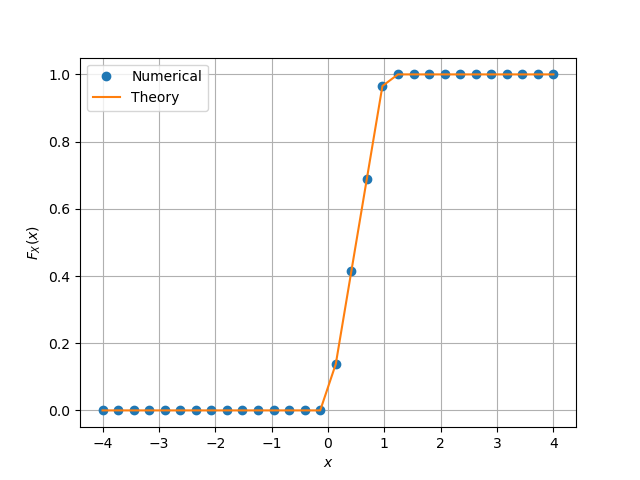
\includegraphics[width=\columnwidth]{figs/cdf_plot_uni.png}
\caption{The CDF of $U$}
\label{fig:uni_cdf}
\end{figure}
%
\item
Find a theoretical expression for $F_{U}(x)$.

\solution As we know \\
Probability density function of U:
\begin{equation}
     P_U(x) = 
    \begin{cases*}
        1 & for $x\in(0,1)$ \\
        0 & otherwise \\
    \end{cases*}
\end{equation}
\begin{align*}
    F_u(x) &= \int_{- \infty }^{x} \pr{U=a} da\\
     &= \int_{- \infty }^{0} (0) da + \int_{0}^{x} (1) da\\
     &= x
\end{align*}
\begin{equation}
    F_u(x) = 
    \begin{cases*}
    0 & for $x<0$\\
    $x$ & for $x \in (0,1)$\\
    1 & for $x>1$
    \end{cases*}
\end{equation}
%	
\item
The mean of $U$ is defined as
%
\begin{equation}
E\sbrak{U} = \frac{1}{N}\sum_{i=1}^{N}U_i
\end{equation}
%
and its variance as
%
    \begin{equation}
        \text{var}\sbrak{U} = E\sbrak{U- E\sbrak{U}}^2 
    \end{equation}
Write a C program to  find the mean and variance of $U$.\\ 
\solution\\
The Mean and Variance of $X$ is plotted in Fig. \ref{fig:mean_variance}
\begin{lstlisting}
wget https://github.com/Pranav-Varma-03/Ai1110-Assig/blob/main/Random%20Numbers/codes/q1_4.c
wget https://github.com/Pranav-Varma-03/Ai1110-Assig/blob/main/Random%20Numbers/codes/coeffs.h
\end{lstlisting}
\begin{figure}[!ht]
\centering
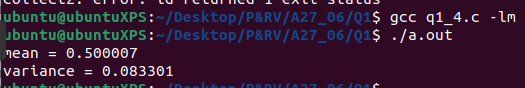
\includegraphics[width=\columnwidth]{figs/q1.png}
\caption{The Mean and Variance of $X$}
\label{fig:mean_variance}
\end{figure}
%
%We get the mean of $U$ as $0.500007$ and the variance of $U$ as $0.083301$.
\item Verify your result theoretically given that
	\begin{equation}
        E\sbrak{U^k} = \int_{-\infty}^{\infty}x^k dF_{U}(x)
    \end{equation}
    \end{enumerate}
%
\solution \\
\begin{enumerate}
    \item k = 1 : E[U] is the mean
    \item k = 2 : E[$U^2$] \\
    where, var[U] = E[$U^2$] - (E[U$])^2$
\end{enumerate}
i) Verifying Mean of sample of $10^6$ Uniform Random Variable
\begin{align*}
    E\sbrak{U} &= \int_{-\infty}^{\infty}xdF_{U}(x)\\
\end{align*}
\begin{equation}
    As,F_{U}(x) = 
    \begin{cases*}
        0 & for $x < 0$ \\
        x & for $x \in (0,1)$\\
        1 & for $x > 1$
    \end{cases*}
\end{equation}
\begin{align*}
    E\sbrak{U} &= 0 + \int_{0}^{1}xd(x) + 0\\[7pt]
    E\sbrak{U} &= \dfrac{x^2}{2} \Big|_0^1\\[7pt]
    E\sbrak{U} &= 0.5
\end{align*}
%
    \begin{align}
        E\sbrak{U} &\approx 0.5
    \end{align}
ii) Verifying Variance of sample of $10^6$ Uniform Random Variable
\begin{align*}
    E\sbrak{U^2} = \int_{-\infty}^{\infty}x^2dF_{U}(x)
\end{align*}
\begin{equation*}
    As,F_{U}(x) = 
    \begin{cases*}
        0 & for $x < 0$ \\
        x & for $x \in (0,1)$\\
        1 & for $x > 1$
    \end{cases*}
\end{equation*}
\begin{align*}
        E\sbrak{U^2} &= 0+\int_{0}^{1}x^2d(x)+0\\
        E\sbrak{U^2} &= \dfrac{x^3}{3} \Big|_0^1\\
        E\sbrak{U^2} &= \dfrac{1}{3} = 0.33 \\
    \end{align*}
Thus,
\begin{align*}
    Var\sbrak{U} &= E\sbrak{U^2} - (E\sbrak{U})^2\\
    Var\sbrak{U} &= (\dfrac{1}{3}) - (\dfrac{1}{2})^2\\
    Var\sbrak{U} &= 0.0833
    \end{align*}
%    
    \begin{align}
        Var\sbrak{U} \approx 0.0833
    \end{align}
\section{Central Limit Theorem}
%
%
\begin{enumerate}[label=\textbf{\thesection.\arabic*},ref=\thesection.\theenumi]
\item
Generate $10^6$ samples of the random variable
%
\begin{equation}
X = \sum_{i=1}^{12}U_i -6
\end{equation}
%
using a C program, where $U_i, i = 1,2,\dots, 12$ are  a set of independent uniform random variables between 0 and 1
and save in a file called gau.dat

\solution Download the following files and execute the  C program.
\begin{lstlisting}
wget https://github.com/Pranav-Varma-03/Ai1110-Assig/blob/main/Random%20Numbers/codes/q1_4.c
wget https://github.com/Pranav-Varma-03/Ai1110-Assig/blob/main/Random%20Numbers/codes/coeffs.h
\end{lstlisting}
%
\item
Load gau.dat in python and plot the empirical CDF of $X$ using the samples in gau.dat. What properties does a CDF have?

\solution The required python file can be downloaded using
\begin{lstlisting}
wget https://github.com/Pranav-Varma-03/Ai1110-Assig/blob/main/Random%20Numbers/codes/q2_4.c
\end{lstlisting}
The CDF of $X$ is plotted in Fig. \ref{fig:gauss_cdf}
\begin{figure}[!ht]
\centering
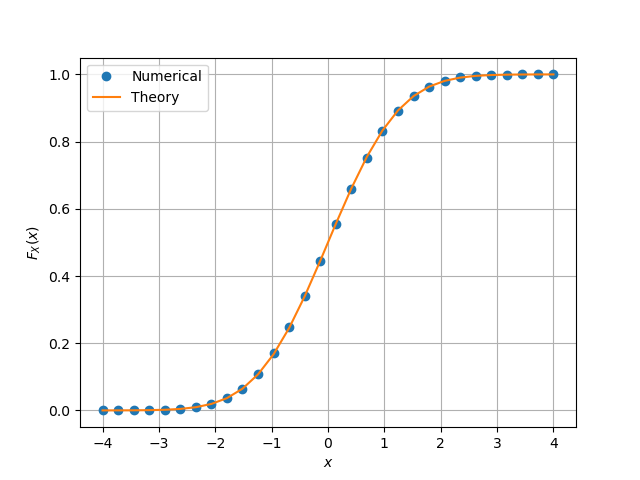
\includegraphics[width=\columnwidth]{figs/cdf_plot_gau.png}
\caption{The CDF of $X$}
\label{fig:gauss_cdf}
\end{figure}
Properties of CDF:
\begin{itemize}
    \item cdf is non decreasing fucntion
    \item $\lim_{x \to -\infty} f(x) = 0$
    \item $\lim_{x \to +\infty} f(x) = 1$
\end{itemize}
%


\item
Load gau.dat in python and plot the empirical PDF of $X$ using the samples in gau.dat. The PDF of $X$ is defined as
\begin{align}
p_{X}(x) = \frac{d}{dx}F_{X}(x)
\end{align}
What properties does the PDF have?\\
\solution The PDF of $X$ is plotted in Fig. \ref{fig:gauss_pdf} using the code below
\begin{lstlisting}
wget https://github.com/Pranav-Varma-03/Ai1110-Assig/blob/main/Random%20Numbers/codes/pdf_plot_gau.py
\end{lstlisting}
Properties of PDF:
\begin{itemize}
    \item It is symmetric about y-axis
    \item Area under curve is 1 i.e., $\int_{-\infty}^{\infty} P_X(x) = 1$
\end{itemize}

\begin{figure}{!ht}
\centering
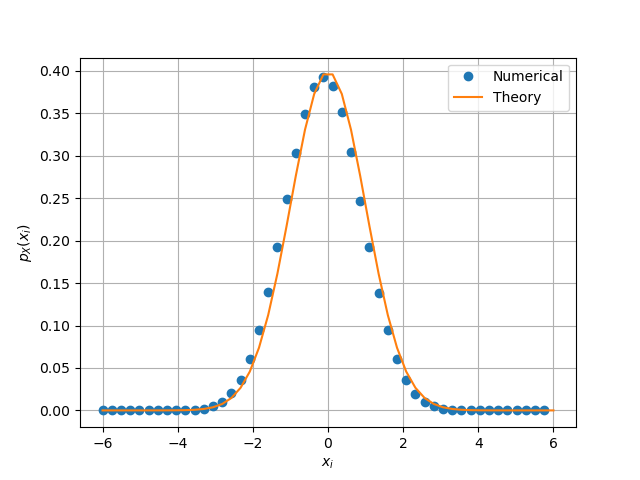
\includegraphics[height=6.5cm,width=\columnwidth]{figs/pdf_plot_gau.png}
\caption{The PDF of $X$}
\label{fig:gauss_pdf}
\end{figure}
%
%
%
\item Find the mean and variance of $X$ by writing a C program.\\
\solution
Execute the C program given below:
\begin{lstlisting}
https://github.com/Pranav-Varma-03/Ai1110-Assig/blob/main/Random%20Numbers/codes/q2_4.c
\end{lstlisting}
%
% 
\ref{fig:mean_variance}
\begin{figure}[!ht]
\centering
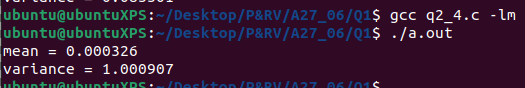
\includegraphics[width=\columnwidth]{figs/q2.png}
\caption{The Mean and Variance of $X$}
\label{fig:mean_variance}
\end{figure}
%
%
%
\item Given that 
\begin{align}
p_{X}(x) = \frac{1}{\sqrt{2\pi}}\exp\brak{-\frac{x^2}{2}}, -\infty < x < \infty,
\label{eq:2.3}
\end{align}
repeat the above exercise theoretically.
%------------------------------------------------------------------------------------
\solution \\
    \begin{equation*}
        E\sbrak{U^k} = \int_{-\infty}^{\infty}x^kdF_{U}(x)\\
    \end{equation*}
%	
	\begin{enumerate}
    		\item k = 1 : E[U] is the mean 
   		\item k = 2 : E[$U^2$] \\[9pt]
    		where, var[U] = E[$U^2$] - (E[U$])^2$\\
	\end{enumerate}
i) Verifying Mean by using \eqref{eq:2.3}:
    \begin{align*}
    		E\sbrak{U} &= \int_{-\infty}^{\infty} x p_X(x)dx\\
    		E\sbrak{U} &= \int_{-\infty}^{\infty} x \frac{1} {\sqrt{2\pi}} \exp\brak{-\frac{x^2}{2}} dx \\[9pt]
   		E\sbrak{U} &= \dfrac{1}{2} \sbrak{ \int_{-\infty}^{\infty} x \frac{1} {\sqrt{2\pi}} \exp\brak{-\frac{x^2}{2}} dx} \\[7pt] &+ \dfrac{1}{2} \sbrak{\int_{-\infty}^{\infty} (-x) \frac{1}{\sqrt{2\pi}} \exp\brak{-\frac{x^2}{2}} dx}\\[9pt]
   		E\sbrak{U} &= 0
    \end{align*}
%
	\begin{align}
        E\sbrak{U} &\approx 0
	\end{align}
%
ii) Verifying Variance by using \eqref{eq:2.3}:
	\begin{align*}
    	 E\sbrak{U^2} &= \int_{-\infty}^{\infty} x^2 p_X(x) dx\\[7pt]
    	 E\sbrak{U^2} &= \int_{-\infty}^{\infty} x^2 \frac{1}{\sqrt{2\pi}}\exp\brak{-\frac{x^2}{2}} dx \\[7pt]
     E\sbrak{U^2} &= 2\int_{0}^{\infty} x^2 \frac{1}{\sqrt{2\pi}}\exp\brak{-\frac{x^2}{2}} dx \\
     E\sbrak{U^2} &= \sqrt{\frac{2}{\pi}} \sbrak{x \exp\brak{-\frac{x^2}{2}} - \int_{0}^{\infty}\exp\brak{ -\frac{x^2}{2}} dx}\\
     E\sbrak{U^2} &= \sqrt{\frac{2}{\pi}} \sbrak{0 + \sqrt{\frac{\pi}{2}}}\\
     E\sbrak{U^2} &= 1
     \end{align*}	
%	
	\begin{align*}
        \therefore Var[U] &=  E\sbrak{U^2} -  (E\sbrak{U})^2\\
        &= 1 - 0\\
        &=1
	\end{align*}
%	
	\begin{align}
    		Var[U] \approx 1
	\end{align}
%---------------------------------------------------------------------------------------------------------
\end{enumerate}
\section{From Uniform to Other}
\begin{enumerate}[label=\textbf{\thesection.\arabic*},ref=\thesection.\theenumi]
%
\item
Generate samples of 
%
\begin{equation}
V = -2\ln\brak{1-U}
\end{equation}
%
and plot its CDF. 
\\
\\
\solution
Execute the following python code
\begin{lstlisting}
wget https://github.com/Pranav-Varma-03/Ai1110-Assig/blob/main/Random%20Numbers/codes/cdf_plot_logg.py
\end{lstlisting}
%
The output CDF is plotted in Figure \eqref{fig:other_cdf}.
\begin{figure}[!ht]
\centering
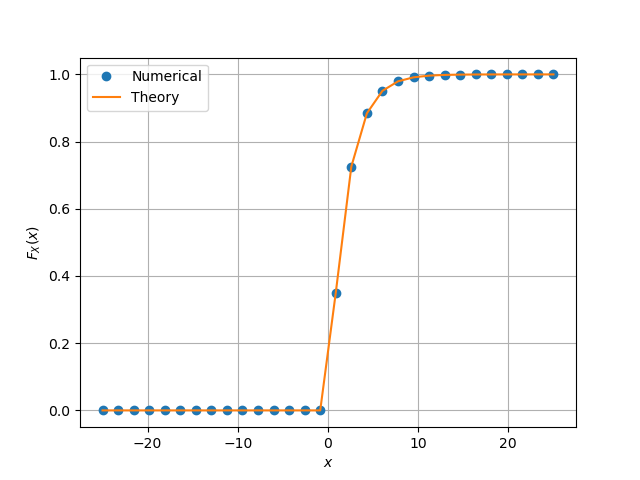
\includegraphics[width=\columnwidth]{figs/cdf_plot_other.png}
\caption{The CDF of $X$}
\label{fig:other_cdf}
\end{figure}
%
%
\item Find a theoretical expression for $F_V(x)$.

\solution\\
Need to find $F_v(x) i.e., \pr{V \le x}$ :
	\begin{align*}
  	   &= \pr{V \le x}\\
  	   &= \pr{-2ln(1-U) \le x}\\
  	   &= \pr{ln(1-U) \ge \frac{-x}{2}} \\
 	   &= \pr{U \le 1 - exp\brak{\frac{-x}{2}}}
	\end{align*}
As we know, $\pr{U \le k} = k$ :
	\begin{align*}
  		\therefore F_V(x) &=  \pr{U \le 1 - exp\brak{\frac{-x}{2}}}\\
  		&= 1 - exp\brak{\frac{-x}{2}}
	\end{align*}
%	
	\begin{equation}
    		As,F_V(x) = 
    		\begin{cases*}
        1 - exp\brak{\frac{-x}{2}} & for $x > 0$ \\
        0 & for $x < 0$
    		\end{cases*}
	\end{equation}
\end{enumerate}
\end{document}